\documentclass[article]{jss}
\usepackage[utf8]{inputenc}

\providecommand{\tightlist}{%
  \setlength{\itemsep}{0pt}\setlength{\parskip}{0pt}}

\author{
Sahir Bhatnagar *\\McGill Univeristy \And Maxime Turgeon *\\McGill University \And James Hanley\\McGill Univeristy \And Olli Saarela\\University of Toronto
}
\title{\pkg{casebase}: An Alternative Framework For Survival Analysis}

\Plainauthor{Sahir Bhatnagar *, Maxime Turgeon *, James Hanley, Olli Saarela}
\Plaintitle{casebase: An Alternative Framework For Survival Analysis}
\Shorttitle{\pkg{casebase}: An Alternative Framework For Survival Analysis}

\Abstract{
The abstract of the article. * joint co-authors
}

\Keywords{keywords, not capitalized, \proglang{Java}}
\Plainkeywords{keywords, not capitalized, Java}

%% publication information
%% \Volume{50}
%% \Issue{9}
%% \Month{June}
%% \Year{2012}
%% \Submitdate{}
%% \Acceptdate{2012-06-04}

\Address{
    Sahir Bhatnagar *\\
  McGill Univeristy\\
  1020 Pine Avenue West Montreal, QC, Canada H3A 1A2\\
  E-mail: \email{sahir.bhatnagar@mail.mcgill.ca}\\
  URL: \url{http://sahirbhatnagar.com/}\\~\\
      Maxime Turgeon *\\
  McGill University\\
  1020 Pine Avenue West Montreal, QC, Canada H3A 1A2\\
  E-mail: \email{maxime.turgeon@mail.mcgill.ca}\\
  URL: \url{http://maxturgeon.ca/}\\~\\
      James Hanley\\
  McGill Univeristy\\
  1020 Pine Avenue West Montreal, QC, Canada H3A 1A2\\
  E-mail: \email{james.hanley@mcgill.ca}\\
  URL: \url{http://www.medicine.mcgill.ca/epidemiology/hanley/}\\~\\
      Olli Saarela\\
  University of Toronto\\
  Dalla Lana School of Public Health, 155 College Street, 6th floor,
  Toronto, Ontario M5T 3M7, Canada\\
  E-mail: \email{olli.saarela@utoronto.ca}\\
  URL: \url{http://individual.utoronto.ca/osaarela/}\\~\\
  }

% Pandoc header

\usepackage{amsmath}

\begin{document}

\section{Code formatting}\label{code-formatting}

Don't use markdown, instead use the more precise latex commands:

\begin{itemize}
\tightlist
\item
  \proglang{Java}
\item
  \pkg{plyr}
\item
  \code{print("abc")}
\end{itemize}

\section{Introduction}\label{introduction}

\begin{itemize}
\tightlist
\item
  Motivation

  \begin{itemize}
  \tightlist
  \item
    Flexible
  \item
    Flexible
  \item
    Flexible
  \end{itemize}
\end{itemize}

\section{Theoretical details}\label{theoretical-details}

As discussed in Hanley \& Miettinen \citeyearpar{hanley2009fitting}, the
key idea behind case-base sampling is to discretize the study base into
an infinite amount of \emph{person moments}. These person moments are
indexed by both an individual in the study and a time point, and
therefore each person moment has a covariate profile, an exposure status
and an outcome status attached to it. We note that there is only a
finite number of person moments associated with the event of interest
(what Hanley \& Miettinen call the \emph{case series}). The case-base
sampling refers to the sampling from the base of a representative finite
sample called the \emph{base series}.

Popular survival analysis methods, like Kaplan-Meier and Cox regression,
rely on the notion of risk-set sampling. Case-base sampling can be seen
as an alternative.

As shown by Saarela \& Arjas \citeyearpar{saarela2015non} (and further
expanded in Saarela \citeyearpar{saarela2016case}), writing the
likelihood arising from this data-generating mechanism using the
framework of non-homogenous Poisson processes, we eventually reach an
expression where each person-moment's contribution is of the form
\[\frac{\lambda(t)^{dN(t)}}{\rho(t) + \lambda(t)},\] where \(N(t)\) is
the counting process associated with the event of interest,
\(\lambda(t)\) is the corresponding hazard function, and \(\rho(t)\) is
the hazard function for the Poisson process associated with case-base
sampling. This parametric form suggests that we can readily estimate
log-hazards of the form \(\log(\lambda(t)) = g(t; X)\) using logistic
regression, where each observation corresponds to a person moment, the
function \(g(t; X)\) is linear in a finite number of parameters, and
where we treat \(\log(\rho(t))\) as an offset.

In Hanley \& Miettinen \citeyearpar{hanley2009fitting}, the authors
suggest performing case-base samping \emph{uniformly}, i.e.~to sample
the base series uniformly from the study base. In terms of Poisson
processes, this sampling strategy corresponds to a time-homogeneous
Poisson process with intensity equal to \(b/B\), where \(b\) is the
number of sampled observations in the base series, and \(B\) is the
total population-time for the study base. More complex examples are also
available; see for example Saarela \& Arjas
\citeyearpar{saarela2015non}, where the probabilities of the sampling
mechanism are proportional to the cardiovascular disease event rate
given by the Framingham score.

\section{Implementation details}\label{implementation-details}

The functions in the casebase package can be divided into two
categories: 1) data visualization, in the form of population-time plots;
and 2) data analysis.

We explicitely aimed at being compatible with both \code{data.frame}s
and \code{data.table}s. This is evident in some of the coding choices we
made, and it is also reflected in our testing units.

\subsection{Population-time plots}\label{population-time-plots}

\subsection{Data analysis}\label{data-analysis}

The data analysis step was separated into three parts: 1) case-base
sampling; 2) estimation of the smooth hazard function; and 3)
calculation of the risk function. By separating the sampling and
estimation functions, we allowed the possibility of users implementing
more complex sampling scheme, as described in Saarela
\citeyearpar{saarela2016case}.

The sampling scheme selected for \code{sampleCaseBase} was described in
Hanley and Miettinen \citeyearpar{hanley2009fitting}: we first sample
along the ``person'' axis, proportional to each individual's total
follow-up time, and then we sample a moment uniformly over their
follow-up time. This sampling scheme is equivalent to the following
picture: imagine representing the total follow-up time of all
individuals in the study along a single dimension, where the follow-up
time of the next individual would start exactly when the follow-up time
of the previous individual ends. Then the base series could be sampled
uniformly from this one-dimensional representation of the overall
follow-up time. In any case, the output is a dataset of the same class
as the input, where each row corresponds to a person-moment. The
covariate profile for each such person-moment is retained, and an offset
term is added to the dataset. This output could then be used to fit a
smooth hazard function, or for visualization of the base series.

The fitting function \code{fitSmoothHazard} starts by looking at the
class of the dataset: if it was generated from \code{sampleCaseBase}, it
automatically inherited the class \code{cbData}. If the dataset supplied
to \code{fitSmoothHazard} does not inherit from \code{cbData}, then the
fitting function starts by calling \code{sampleCaseBase} to generate the
base series. In other words, the occasional user can bypass
\code{sampleCaseBase} altogether and only worry about the fitting
function \code{fitSmoothHazard}.

The fitting function retains the familiar formula interface of
\code{glm}. The left-hand side of the formula should be the name of the
column corresponding to the event type. The right-hand side can be any
combination of the covariates, along with an explicit functional form
for the time variable. Note that non-proportional hazard models can be
achieved at this stage by adding an interaction term involving time. The
offset term does not need to be specified by the user, as it is
automatically added to the formula.

Finally, the hazard function is fitted to the data using the function
\code{glm}, unless there is more than one type event (i.e.~in a
competing-risk analysis), in which case it uses the multinomical
regression capabilities of the \pkg{VGAM} package. This package was
selected for its ability to fit multinomial regression models with an
offset.

Once a model-fit object has been returned by \code{fitSmoothHazard}, all
the familiar summary and diagnostic functions are available:
\code{print}, \code{summary}, \code{predict}, \code{plot}, etc. Our
package provides one more functionality: it computes risk functions from
the model fit. For the case of a single event, it uses the familiar
identity \[S(t) = \exp\left(-\int_0^t h(u;X) du\right).\] The integral
is computed using either the \code{stats::integrate} function or
Monte-Carlo integration. For the case of a competing-event analysis, the
event-specific risk is computed using a nested double integral; in this
setting, Monte-Carlo integration is faster and more flexible than
\code{stats::integrate}. This is due to the fact that the computation
involves a double loop over the selected time points; Monte-Carlo
integration performs this step by using the vectorized \code{rowSums}
and \code{colSums} functions.

To decide between a single-event and a competing-event analysis, we
created \code{absoluteRisk} as an \code{S3} generic, with methods for
both \code{glm} and \code{CompRisk} objects (the latter inherits from
\code{vglm} as well). The method dispatch system of \proglang{R} then
takes care of matching the correct input to the correct methodology,
without the user's intervention.

\section{Case study 1: Veteran data (or ERSPC if we
can)}\label{case-study-1-veteran-data-or-erspc-if-we-can}

\begin{itemize}
\tightlist
\item
  First example
\item
  Show how we can test for non-proportional hazard?
\end{itemize}

\section{Case study 2: Bone-marrow
transplant}\label{case-study-2-bone-marrow-transplant}

The next example shows how case-base sampling can also be used in the
context of a competing risk analysis. For illustrative purposes, we will
use the same data that was used in Scrucca \emph{et al}
\citeyearpar{scrucca2010regression}. The data was downloaded from the
main author's website, and it is also available as part of the
\pkg{casebase} package.

\begin{CodeChunk}

\begin{CodeInput}
R> library(casebase)
R> data(bmtcrr)
\end{CodeInput}
\end{CodeChunk}

The data contains information on 177 patients who received a stem-cell
transplant for acute leukemia. The event of interest is relapse, but
other competing causes (e.g.~transplant-related death) were also
recorded Several covariates were also captured at baseline: sex, disease
type (acute lymphoblastic or myeloblastic leukemia, abbreviated as ALL
and AML, respectively), disease phase at transplant (Relapse, CR1, CR2,
CR3), source of stem cells (bone marrow and peripheral blood, coded as
BM+PB, or only peripheral blood, coded as PB), and age. A summary of
these baseline characteristics appear in Table \ref{tab:table1bmtcrr}.
We note that the statistical summaries were generated differently for
different variable types: for continuous variables, we gave the range,
followed by the mean and standard deviation; for categorical variables,
we gave the counts for each category.

\begin{table}[ht]
\centering
\begin{tabular}{lll}
  \hline
Variable & Description & Statistical summary \\ 
  \hline
Sex & Sex & M=Male (100) \\ 
   &  & F=Female (77) \\ 
  D & Disease & ALL (73) \\ 
   &  & AML (104) \\ 
  Phase & Phase & CR1 (47) \\ 
   &  & CR2 (45) \\ 
   &  & CR3 (12) \\ 
   &  & Relapse (73) \\ 
  Source & Type of transplant & BM+PB (21) \\ 
   &  & PB (156) \\ 
  Age & Age of patient (years) & 4–62 \\ 
   &  & 30.47 (13.04) \\ 
  Ftime & Failure time (months) & 0.13–131.77 \\ 
   &  & 20.28 (30.78) \\ 
  Status & Status indicator & 0=censored (46) \\ 
   &  & 1=relapse (56) \\ 
   &  & 2=competing event (75) \\ 
   \hline
\end{tabular}
\caption{Baseline characteristics of patients in the stem-cell transplant study.}
\label{tab:table1bmtcrr}
\end{table}

In order to try and visualize the incidence density of relapse, we can
look at the corresponding population-time plot. In Figure
\ref{fig:compPop1}, failure times associated with relapse are
highlighted on the plot using red points, while Figure
\ref{fig:compPop2} provides a similar population-time plot for competing
events.

\begin{CodeChunk}
\begin{figure}

{\centering 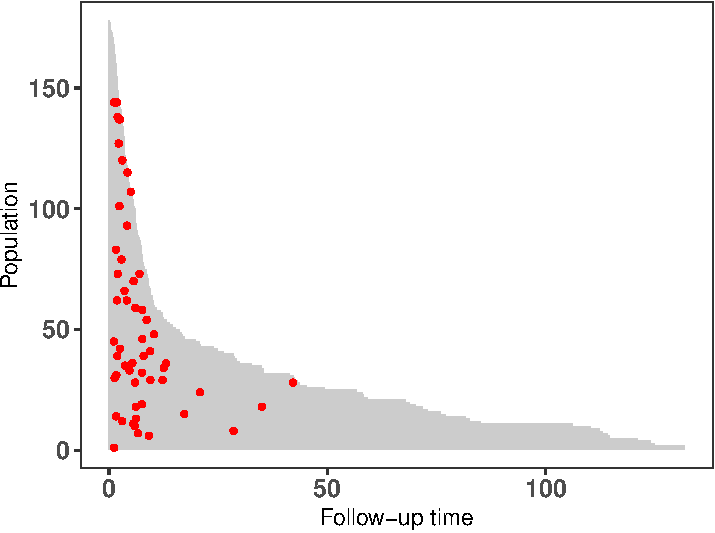
\includegraphics{casebase_jss_files/figure-latex/compPop1-1} 

}

\caption{\label{fig:compPop1}Population-time plot for the stem-cell transplant study. The points represent the event of interest (i.e., relapse).}\label{fig:compPop1}
\end{figure}
\end{CodeChunk}

\begin{CodeChunk}
\begin{figure}

{\centering 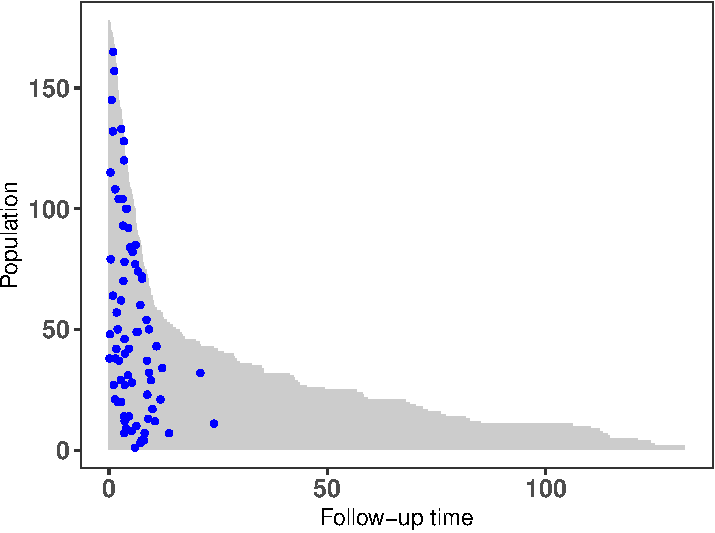
\includegraphics{casebase_jss_files/figure-latex/compPop2-1} 

}

\caption{\label{fig:compPop2}Population-time plot for the stem-cell transplant study. The points represent the competing events.}\label{fig:compPop2}
\end{figure}
\end{CodeChunk}

Our main objective is to compute the absolute risk of relapse for a
given set of covariates. First, we fit a smooth hazard to the data; for
the sake of this example, we opted for a linear term for time:

\begin{CodeChunk}

\begin{CodeInput}
R> model_cb <- fitSmoothHazard(
R+     Status ~ ftime + Sex + D + Phase + Source + Age, 
R+     data = bmtcrr, 
R+     ratio = 100, 
R+     time = "ftime")
\end{CodeInput}
\end{CodeChunk}

From the fit object, we can extract both the hazard ratios and their
corresponding confidence intervals:

\begin{CodeChunk}

\begin{tabular}{l|r|l}
\hline
Covariates & HR & 95\% CI\\
\hline
Sex & 0.82 & (0.46, 1.48)\\
\hline
Disease & 0.48 & (0.25, 0.92)\\
\hline
Phase (CR2 vs. CR1) & 1.43 & (0.56, 3.66)\\
\hline
Phase (CR3 vs. CR1) & 1.63 & (0.41, 6.45)\\
\hline
Phase (Relapse vs. CR1) & 4.73 & (2.13, 10.48)\\
\hline
Source & 1.51 & (0.49, 4.69)\\
\hline
Age & 0.99 & (0.97, 1.02)\\
\hline
\end{tabular}

\end{CodeChunk}

As we can see, the only significant hazard ratio is the one associated
with the phase of the disease at transplant. More precisely, being in
relapse at transplant is associated with a hazard ratio of 3.92 when
compared to CR1.

Given our estimate of the hazard function, we can compute the absolute
risk curve for a fixed covariate profile. We performed this computation
for a 35 year old woman who received a stem-cell transplant from
peripheral blood at relapse. We compared the absolute risk curve for
such a woman with acute lymphoblastic leukemia with that for a similar
woman with acute myeloblastic leukemia. Figure \ref{fig:compAbsrisk}
shows these two curves as a function of time. This figure also shows the
Kaplan-Meier estimate fitted to the two disease groups (ignoring the
other covariates).

\begin{CodeChunk}

\begin{CodeInput}
R> # Pick 100 equidistant points between 0 and 60 months
R> time_points <- seq(0, 60, length.out = 100)
R> 
R> # Data.frame containing risk profile
R> newdata <- data.frame("Sex" = factor(c("F", "F"), 
R+                                      levels = levels(bmtcrr[,"Sex"])),
R+                       "D" = c("ALL", "AML"),
R+                       "Phase" = factor(c("Relapse", "Relapse"), 
R+                                        levels = levels(bmtcrr[,"Phase"])),
R+                       "Age" = c(35, 35),
R+                       "Source" = factor(c("PB", "PB"), 
R+                                         levels = levels(bmtcrr[,"Source"])))
R> 
R> # Estimate absolute risk curve
R> risk_cb <- absoluteRisk(object = model_cb, time = time_points,
R+                         method = "montecarlo", newdata = newdata)
\end{CodeInput}
\end{CodeChunk}

\begin{CodeChunk}
\begin{figure}

{\centering \includegraphics{casebase_jss_files/figure-latex/unnamed-chunk-6-1} 

}

\caption{\label{fig:compAbsrisk}Absolute risk curve for a fixed covariate profile and the two disease groups. The estimate obtained from case-base sampling is compared to the Kaplan-Meier estimate.}\label{fig:unnamed-chunk-6}
\end{figure}
\end{CodeChunk}

\section{Case study 3: Vaccination study (recurrent
events)}\label{case-study-3-vaccination-study-recurrent-events}

\begin{itemize}
\tightlist
\item
  Give a more complex example of sampling; time-dependent exposure

  \begin{itemize}
  \tightlist
  \item
    Sampling needs to be done manually, but fitting function can still
    be used
  \end{itemize}
\end{itemize}

\renewcommand\refname{Discussion}
\bibliography{casebase_references.bib}


\end{document}

